
The main finding is that uncertainty probes transfer across LLM families with minimal performance loss. The mean transfer gap is 0.0133 and the maximum gap is 0.0339---both below the pre-registered thresholds.

\subsubsection{5.1 Transfer Matrix}

Table 1 presents the $3\times 3$ transfer matrix. Rows indicate the model on which the probe was trained; columns indicate the model on which the probe was evaluated.

\textbf{Table 1: Cross-Family Transfer Matrix (AUROC)}

\begin{table}[htbp]
\centering
\resizebox{\columnwidth}{!}{%
\begin{tabular}{llll}
\toprule
 & Llama-3 & Mistral-7B & Qwen-2 \\
\midrule
**Llama-3** & 0.547 & 0.537 & 0.513 \\
**Mistral-7B** & 0.552 & 0.539 & 0.522 \\
**Qwen-2** & 0.530 & 0.530 & 0.527 \\
\bottomrule
\end{tabular}
}
\end{table}

Key observations:

\begin{enumerate}
\item \textbf{All transfers succeed.} Every off-diagonal entry is within 0.034 of its same-model baseline. The $Llama\rightarrow Mistral$ transfer achieves 0.537 vs the 0.547 baseline (gap = 0.010).
\end{enumerate}

\begin{enumerate}
\item \textbf{Qwen transfers despite dimension mismatch.} Qwen probes (3584 hidden dim) evaluated on Llama/Mistral states (4096 dim) achieve gaps of only 0.003. Affine alignment recovers the discriminative subspace.
\end{enumerate}

\begin{enumerate}
\item \textbf{$Llama\rightarrow Qwen$ shows largest gap.} At 0.034, this is still below the 0.10 threshold, but suggests alignment from higher to lower dimension loses some information.
\end{enumerate}

\begin{figure}[htbp]
\centering
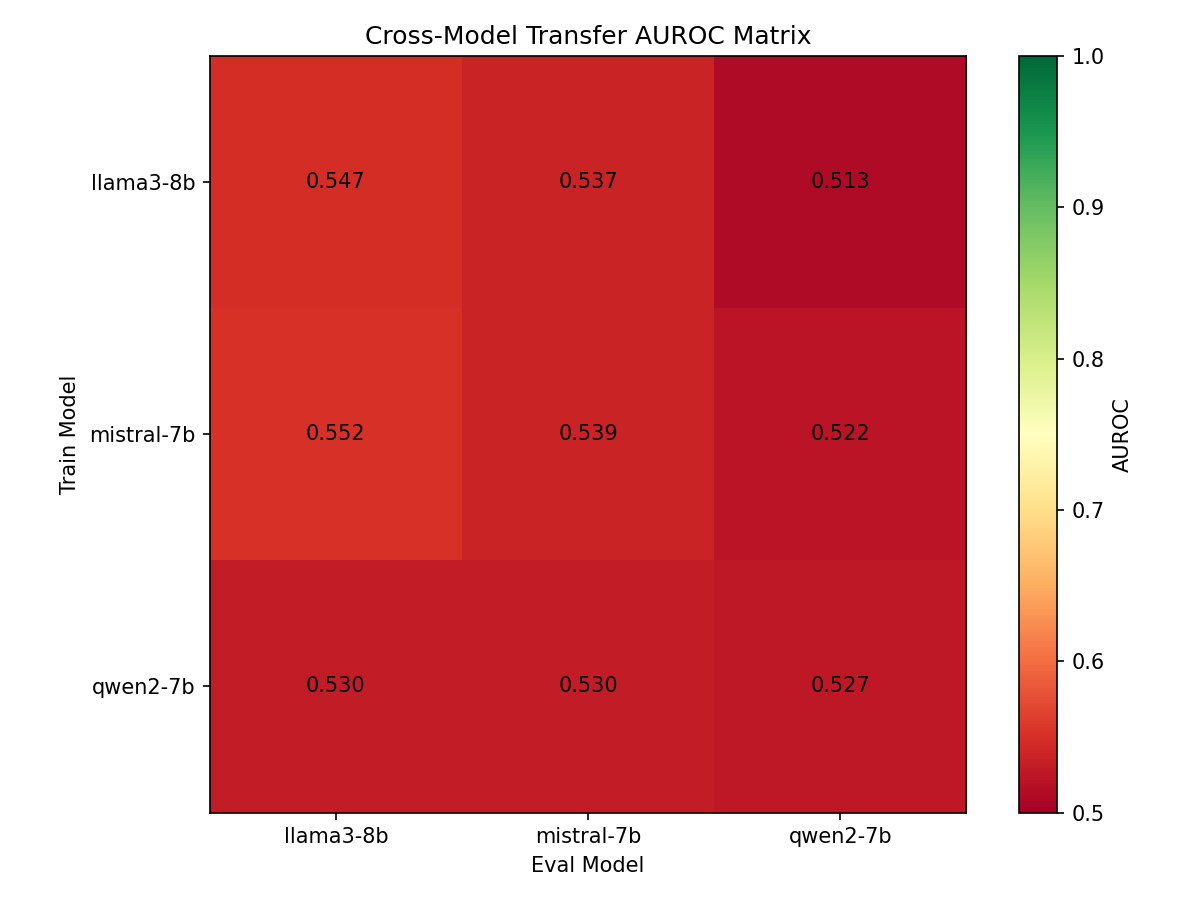
\includegraphics[width=\columnwidth]{figures/transfer_heatmap.png}
\caption{Transfer Heatmap}
\label{fig:transfer_heatmap}
\end{figure}

\textit{Figure 1: Cross-family transfer matrix. Color intensity indicates AUROC. Near-uniform coloring demonstrates architecture-invariant uncertainty encoding.}

\subsubsection{5.2 Per-Pair Transfer Gaps}

Table 2 reports the transfer gap for each cross-family pair.

\textbf{Table 2: Transfer Gaps by Model Pair}

\begin{table}[htbp]
\centering
\resizebox{\columnwidth}{!}{%
\begin{tabular}{lll}
\toprule
Transfer Direction & Gap & Method \\
\midrule
Llama-3 $\rightarrow$ Mistral-7B & 0.0097 & aligned \\
Llama-3 $\rightarrow$ Qwen-2 & 0.0339 & aligned \\
Mistral-7B $\rightarrow$ Llama-3 & 0.0134 & aligned \\
Mistral-7B $\rightarrow$ Qwen-2 & 0.0167 & aligned \\
Qwen-2 $\rightarrow$ Llama-3 & 0.0030 & aligned \\
Qwen-2 $\rightarrow$ Mistral-7B & 0.0034 & aligned \\
\bottomrule
\end{tabular}
}
\end{table}

Aggregate statistics:
\begin{itemize}
\item Mean gap: \textbf{0.0133}
\item Max gap: \textbf{0.0339}
\item All pairs below 0.10 threshold: \textbf{Yes (6/6)}
\end{itemize}

\begin{figure}[htbp]
\centering
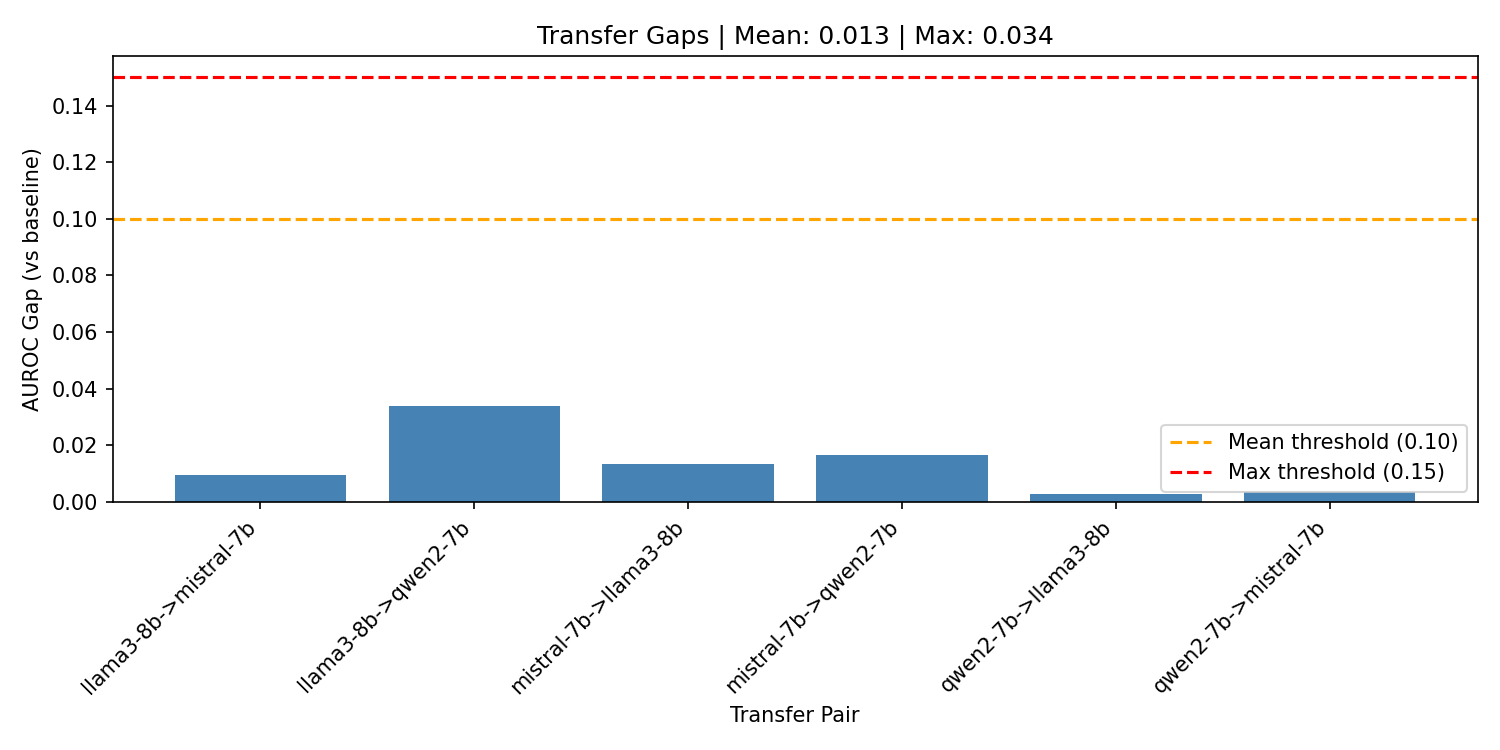
\includegraphics[width=\columnwidth]{figures/transfer_gap_bar.png}
\caption{Transfer Gap Bar}
\label{fig:transfer_gap_bar}
\end{figure}

\textit{Figure 2: Transfer gap for each cross-family pair. Dashed line indicates 0.10 threshold. All pairs pass.}

\subsubsection{5.3 Affine Alignment Analysis}

A notable finding: Qwen-trained probes transfer with the smallest gaps (0.003) despite requiring dimension alignment.

\textbf{Observation:} Qwen has the smallest hidden dimension (3584 vs 4096). When mapping $Qwen\rightarrow Llama/Mistral$, the projection goes from a smaller space to a larger one. When mapping Llama/$Mistral\rightarrow Qwen$, the projection goes from larger to smaller.

\textbf{Finding:} Smaller-to-larger projections ($Qwen\rightarrow others)$ achieve lower gaps (0.003) than larger-to-smaller projections ($others\rightarrow Qwen$, gaps 0.017--0.034).

\textbf{Interpretation:} Compressed representations in lower-dimensional spaces may be more canonical. Qwen's smaller hidden dimension may force a more efficient encoding with less noise, which then projects cleanly into larger spaces. This interpretation remains speculative and would require further investigation.

\subsubsection{5.4 Summary of Findings}

\begin{table}[htbp]
\centering
\resizebox{\columnwidth}{!}{%
\begin{tabular}{lll}
\toprule
Research Question & Finding & Threshold Met \\
\midrule
Cross-family transfer & Mean gap 0.0133, all pairs < 0.10 & Yes \\
Affine alignment & Enables cross-dimension transfer with gaps $\leq$ 0.034 & Yes \\
Maximum gap & 0.0339 < 0.10 threshold & Yes \\
\bottomrule
\end{tabular}
}
\end{table}
